\documentclass[a4paper,12pt]{article}
\usepackage{graphicx}
\usepackage{amsmath,amssymb,amsthm}
\usepackage{geometry}
\usepackage{float}
\usepackage{tikz}
\usepackage{circuitikz}
\usepackage[section]{placeins}

\geometry{margin=1in}

\title{Scientific Calculator Using AVR-GCC}
\author{EE24BTECH11002 - Agamjot Singh}
\date{\today}

\begin{document}

\maketitle

\section*{Features}
\begin{itemize}
    \item Basic operations: addition $(+),$ subtraction $(-),$ multiplication $(*)$, division $(/),$ and power $($\textasciicircum$)$
    \item Trigonometric functions: $\sin$, $\cos$, $\tan$, $\sin^{-1}$ or $\arcsin$, $\cos^{-1}$ or $\arccos$, $\tan^{-1}$ or $\arctan$
    \item Logarithmic functions: natural log ($\ln$), log base 10 ($\log$)
    \item BODMAS implementation using the Shunting Yard Algorithm
    \item Constants: $\pi$, $e$
    \item Memory recall functionality (with EEPROM)
    \item Movable Cursor
\end{itemize}


\subsection*{Components and Circuit Schematic}

\begin{table}[H]
\centering
\begin{tabular}{|c|l|}
\hline
\textbf{Quantity} & \textbf{Component} \\
\hline
1 & Arduino Uno\\
\hline
25 & Push buttons \\
\hline
1 & LCD (16 x 2) \\
\hline
- & Wires \\
\hline
1 & Potentiometer \\
\hline
\end{tabular}
\caption{Materials Required}
\label{tab:materials}
\end{table}

$5 \times 5$ button matrix is built for input from the 25 buttons, which is made to reduce the amount of wires needed to mere 10 wires for 25 buttons. Button matrix connections to the arduino and connections are given below.

\begin{figure}[!ht]
\centering
\resizebox{0.8\textwidth}{!}{%
\begin{circuitikz}
\tikzstyle{every node}=[font=\large]
\draw (4.25,12) to[short] (4.25,6.25);
\draw (4.25,11.25) to[push button] (6.25,11.25);
\draw (4.25,10.25) to[push button] (6.25,10.25);
\draw (4.25,9) to[push button] (6.25,9);
\draw (4.25,7.75) to[push button] (6.25,7.75);
\draw (4.25,6.5) to[push button] (6.25,6.5);
\draw (7,12) to[short] (7,6.25);
\draw (7,11.25) to[push button] (9,11.25);
\draw (7,10.25) to[push button] (9,10.25);
\draw (7,9) to[push button] (9,9);
\draw (7,7.75) to[push button] (9,7.75);
\draw (7,6.5) to[push button] (9,6.5);
\draw (9.75,12) to[short] (9.75,6.25);
\draw (9.75,11.25) to[push button] (11.75,11.25);
\draw (9.75,10.25) to[push button] (11.75,10.25);
\draw (9.75,9) to[push button] (11.75,9);
\draw (9.75,7.75) to[push button] (11.75,7.75);
\draw (9.75,6.5) to[push button] (11.75,6.5);
\draw (12.5,12) to[short] (12.5,6.25);
\draw (12.5,11.25) to[push button] (14.5,11.25);
\draw (12.5,10.25) to[push button] (14.5,10.25);
\draw (12.5,9) to[push button] (14.5,9);
\draw (12.5,7.75) to[push button] (14.5,7.75);
\draw (12.5,6.5) to[push button] (14.5,6.5);
\draw (1.5,12) to[short] (1.5,6.25);
\draw (1.5,11.25) to[push button] (3.5,11.25);
\draw (1.5,10.25) to[push button] (3.5,10.25);
\draw (1.5,9) to[push button] (3.5,9);
\draw (1.5,7.75) to[push button] (3.5,7.75);
\draw (1.5,6.5) to[push button] (3.5,6.5);
\draw (6.25,12.5) to[short] (6.25,6.25);
\draw (6.25,13.5) to[short] (6.25,11.25);
\draw (3.5,12.75) to[short] (0.75,12.75);
\draw (6.25,13.5) to[short] (0.75,13.5);
\draw (11.75,15) to[short] (0.75,15);
\draw (0.75,14.25) to[short] (9,14.25);
\draw (9,14.25) to[short] (9,6.25);
\draw (14.5,15.75) to[short] (0.75,15.75);
\draw [ color={rgb,255:red,255; green,56; blue,56}, ](1.5,11.25) to[short] (0.75,11.25);
\draw [ color={rgb,255:red,240; green,51; blue,51}, ](1.5,10.25) to[short] (0.75,10.25);
\draw [ color={rgb,255:red,229; green,56; blue,56}, ](1.5,9) to[short] (0.75,9);
\draw [ color={rgb,255:red,246; green,49; blue,49}, ](1.5,7.75) to[short] (0.75,7.75);
\draw [ color={rgb,255:red,236; green,50; blue,50}, ](1.5,6.5) to[short] (0.75,6.5);
\node at (1.5,11.25) [circ] {};
\node at (1.5,10.25) [circ] {};
\node at (1.5,9) [circ] {};
\node at (1.5,7.75) [circ] {};
\node at (1.5,6.5) [circ] {};
\node at (3.5,11.25) [circ] {};
\node at (3.5,10.25) [circ] {};
\node at (3.5,9) [circ] {};
\node at (3.5,7.75) [circ] {};
\node at (3.5,6.5) [circ] {};
\node at (4.25,11.25) [circ] {};
\node at (4.25,10.25) [circ] {};
\node at (4.25,9) [circ] {};
\node at (4.25,7.75) [circ] {};
\node at (4.25,6.5) [circ] {};
\node at (6.25,6.5) [circ] {};
\node at (6.25,7.75) [circ] {};
\node at (6.25,9) [circ] {};
\node at (6.25,10.25) [circ] {};
\node at (6.25,11.25) [circ] {};
\node at (7,11.25) [circ] {};
\node at (7,10.25) [circ] {};
\node at (7,9) [circ] {};
\node at (7,7.75) [circ] {};
\node at (7,6.5) [circ] {};
\node at (9,11.25) [circ] {};
\node at (9,10.25) [circ] {};
\node at (9,9) [circ] {};
\node at (9,7.75) [circ] {};
\node at (9,6.5) [circ] {};
\node at (11.75,11.25) [circ] {};
\node at (9.75,11.25) [circ] {};
\node at (9.75,10.25) [circ] {};
\node at (9.75,9) [circ] {};
\node at (9.75,7.75) [circ] {};
\node at (9.75,6.5) [circ] {};
\node at (11.75,6.5) [circ] {};
\node at (11.75,7.75) [circ] {};
\node at (11.75,9) [circ] {};
\node at (11.75,10.25) [circ] {};
\node at (12.5,11.25) [circ] {};
\node at (12.5,10.25) [circ] {};
\node at (12.5,9) [circ] {};
\node at (12.5,7.75) [circ] {};
\node at (12.5,6.5) [circ] {};
\node at (14.5,6.5) [circ] {};
\node at (14.5,7.75) [circ] {};
\node at (14.5,9) [circ] {};
\node at (14.5,10.25) [circ] {};
\node at (14.5,11.25) [circ] {};
\draw [ color={rgb,255:red,255; green,51; blue,51}, ](1.75,11.25) to[short] (1.75,10.75);
\draw [ color={rgb,255:red,255; green,51; blue,51}, ](1.75,10.75) to[short] (13,10.75);
\draw [ color={rgb,255:red,221; green,44; blue,44}, ](13,11.25) to[short] (13,10.75);
\draw [ color={rgb,255:red,255; green,51; blue,51}, ](4.75,10.75) to[short] (4.75,11.25);
\draw [ color={rgb,255:red,255; green,51; blue,51}, ](7.5,10.75) to[short] (7.5,11.25);
\draw [ color={rgb,255:red,255; green,51; blue,51}, ](10.25,10.75) to[short] (10.25,11.25);
\draw [ color={rgb,255:red,255; green,51; blue,51}, ](1.75,10.25) to[short] (1.75,9.5);
\draw [ color={rgb,255:red,248; green,53; blue,53}, ](1.75,9.5) to[short] (13,9.5);
\draw [ color={rgb,255:red,255; green,51; blue,51}, ](13,9.5) to[short] (13,10.25);
\draw [ color={rgb,255:red,245; green,50; blue,50}, ](10.25,10.25) to[short] (10.25,9.5);
\draw [ color={rgb,255:red,233; green,47; blue,47}, ](7.5,10.25) to[short] (7.5,9.5);
\draw [ color={rgb,255:red,220; green,46; blue,46}, ](4.75,10.25) to[short] (4.75,9.5);
\draw [ color={rgb,255:red,251; green,50; blue,50}, ](1.75,9) to[short] (1.75,8.25);
\draw [ color={rgb,255:red,245; green,50; blue,50}, ](1.75,8.25) to[short] (13,8.25);
\draw [ color={rgb,255:red,238; green,58; blue,58}, ](13,9) to[short] (13,8.25);
\draw [ color={rgb,255:red,248; green,53; blue,53}, ](10.25,9) to[short] (10.25,8.25);
\draw [ color={rgb,255:red,253; green,53; blue,53}, ](7.5,9) to[short] (7.5,8.25);
\draw [ color={rgb,255:red,230; green,51; blue,51}, ](4.75,9) to[short] (4.75,8.25);
\draw [ color={rgb,255:red,255; green,51; blue,51}, ](1.75,7.75) to[short] (1.75,7);
\draw [ color={rgb,255:red,255; green,51; blue,51}, ](1.75,7) to[short] (13,7);
\draw [ color={rgb,255:red,234; green,57; blue,57}, ](13,7) to[short] (13,7.75);
\draw [ color={rgb,255:red,227; green,49; blue,49}, ](10.25,7.75) to[short] (10.25,7);
\draw [ color={rgb,255:red,240; green,56; blue,56}, ](7.5,7.75) to[short] (7.5,7);
\draw [ color={rgb,255:red,238; green,68; blue,68}, ](4.75,7.75) to[short] (4.75,7);
\draw [ color={rgb,255:red,255; green,51; blue,51}, ](1.75,6.5) to[short] (1.75,5.75);
\draw [ color={rgb,255:red,233; green,63; blue,63}, ](1.75,5.75) to[short] (13,5.75);
\draw [ color={rgb,255:red,229; green,56; blue,56}, ](13,6.5) to[short] (13,5.75);
\draw [ color={rgb,255:red,225; green,61; blue,61}, ](10.25,6.5) to[short] (10.25,5.75);
\draw [ color={rgb,255:red,236; green,65; blue,65}, ](7.5,6.5) to[short] (7.5,5.75);
\draw [ color={rgb,255:red,242; green,54; blue,54}, ](4.75,6.5) to[short] (4.75,5.75);
\node at (0.75,12.75) [circ] {};
\node at (0.75,13.5) [circ] {};
\node at (0.75,14.25) [circ] {};
\node at (0.75,15) [circ] {};
\node at (0.75,15.75) [circ] {};
\node at (0.75,11.25) [squarepole, color={rgb,255:red,236; green,65; blue,65}] {};
\node at (0.75,10.25) [squarepole, color={rgb,255:red,236; green,65; blue,65}] {};
\node at (0.75,9) [squarepole, color={rgb,255:red,236; green,65; blue,65}] {};
\node at (0.75,7.75) [squarepole, color={rgb,255:red,236; green,65; blue,65}] {};
\node at (0.75,6.5) [squarepole, color={rgb,255:red,236; green,65; blue,65}] {};
\node [font=\large] at (0,15.75) {$D2$};
\node [font=\large] at (0,15) {$D3$};
\node [font=\large] at (0,14.25) {$D4$};
\node [font=\large] at (0,13.5) {$D5$};
\node [font=\large] at (0,12.75) {$D6$};
\node [font=\large] at (0.25,11.25) {$A0$};
\node [font=\large] at (0.25,10.25) {$A1$};
\node [font=\large] at (0.25,9) {$A2$};
\node [font=\large] at (0.25,7.75) {$A3$};
\node [font=\large] at (0.25,6.5) {$A4$};
\draw (11.75,15) to[short] (11.75,6.25);
\draw (14.5,15.75) to[short] (14.5,6.25);
\draw (3.5,12.75) to[short] (3.5,6.25);
\end{circuitikz}
}%

\label{fig:button_matrix}
\caption{Button Matrix Circuit Schematic}
\end{figure}
\FloatBarrier

Note that D2, D3, $\dots$ D6 and A0, A1, $\dots$, A4 are the Arduino's Digital pins and Analog Pins respectively.

\begin{table}[htbp]
    \centering
    \label{tab:arduino-lcd}
    \begin{tabular}{|l|c|l|l|}
        \hline
        \textbf{Arduino} & \textbf{LCD} & \textbf{LCD Pin} & \textbf{LCD Pin} \\
        \textbf{Pins} & \textbf{Pins} & \textbf{Label} & \textbf{Description} \\
        \hline
        GND & 1 & GND & \\
        \hline
        5V & 2 & Vcc & \\
        \hline
        GND & 3 & Vee & Contrast \\
        \hline
        D12 & 4 & RS & Register Select \\
        \hline
        GND & 5 & R/W & Read/Write \\
        \hline
        D11 & 6 & EN & Enable \\
        \hline
        D5 & 11 & DB4 & Serial Connection \\
        \hline
        D4 & 12 & DB5 & Serial Connection \\
        \hline
        D3 & 13 & DB6 & Serial Connection \\
        \hline
        D2 & 14 & DB7 & Serial Connection \\
        \hline
        5V & 15 & LED+ & Backlight \\
        \hline
        GND & 16 & LED- & Backlight \\
        \hline
    \end{tabular}
    \caption{Arduino to LCD Pin Connections}
\end{table}
\FloatBarrier

The schematic for connections is as shown below,
\begin{figure}[H]
    \centering
    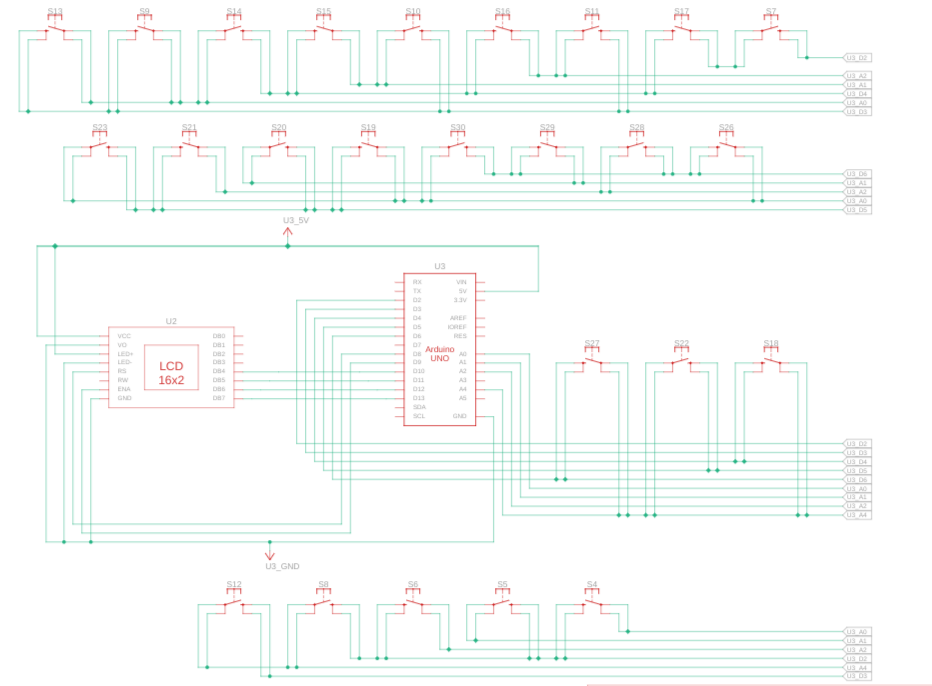
\includegraphics[width=\textwidth]{./figs/schematic.png}
    \caption{Schematic of Circuit.}
    \label{fig:circuit_schematic}
\end{figure}

\section*{Code implementation}
The code is implemented using AVR GCC.
\begin{itemize}
    \item $5\times 5$ button matrix is implemented to check which key is pressed
    \item Parsing the input using the Shunting Yard algorithm
    \item Evaluating result Reversed Polish Expression to a result to display.
    \item Support for functions like trigonometric functions and inverse trigonometric functions, logarithms.
    \item All function implementations are done \textbf{without using math.h} library, solving differential equations by RK4 method.
\end{itemize}

Further Explanation on shunting Yard algorithm is found in the pdf in this directory.

\section*{Explanation of Implementation}
\subsection*{Button Matrix}
The button matrix is a grid of push-button switches arranged in rows and columns. It allows multiple buttons to be connected to the microcontroller using fewer pins. In my circuit, the rows are connected to analog pins (A0 to A4), while the columns are connected to digital pins (D2 to D6) of the Arduino.
\begin{itemize}
    \item The microcontroller scans the matrix by activating each row (setting it HIGH) one at a time while reading the columns for signals.
    \item When a button is pressed, it completes the circuit between its corresponding row and column.
    \item By identifying which row and column are active, the microcontroller determines which button was pressed.
    \item Suppose the first column is set to $ \text{HIGH} $, and a button (unknown to the circuit) is pressed. When reading from the rows, the microcontroller detects a signal from the second row. This confirms that the button pressed is the second button in the first column.
\end{itemize}
This idea helped us reduce the number of pins required to implement a calculator with $25$ buttons to a mere $10$ pins of the microcontroller.

\section*{Numerical Methods}
All the functions are implemented using the RK4 Method.

\subsubsection*{Runge-Kutta 4th Order (RK4) Method}

The RK4 method is given by the following iterative steps to solve the differential equation $ \frac{dy}{dx} = f(x, y) $:
\begin{align}
k_1 = h f(x_n, y_n)
\end{align}
\begin{align}
k_2 = h f\left( x_n + \frac{h}{2}, y_n + \frac{k_1}{2} \right)
\end{align}
\begin{align}
k_3 = h f\left( x_n + \frac{h}{2}, y_n + \frac{k_2}{2} \right)
\end{align}
\begin{align}
k_4 = h f(x_n + h, y_n + k_3)
\end{align}
\begin{align}
y_{n+1} = y_n + \frac{1}{6} \left( k_1 + 2k_2 + 2k_3 + k_4 \right)
\end{align}
where $ h $ is the step size, $ y_n $ is the value of the solution at time $ x_n $, and $ f(x, y) $ represents the differential equation.

\subsubsection*{Trigonometric Functions}
We solve the following differential equation whose solution is $ y(x) = \sin(x) $,
\begin{align}
\frac{d^2y}{dx} + y = 0;
\end{align}
Once we have $\sin{x}$, we can calculate $\cos{x}$ and $\tan{x}$,
\begin{align*} 
 \cos(x) &= \sin \left( \frac{\pi}{2} - x \right)\\ 
 \tan(x) &= \frac{\sin(x)}{\cos(x)}
\end{align*}

\subsubsection*{Inverse Trigonometric Functions}

We solve the differential equation whose solution is $ y(x) = \arcsin(x) $,
\begin{align}
\frac{dy}{dx} = \frac{1}{\sqrt{1 - x^2}}
\end{align}
Once we have $\arcsin(x)$, we can calculate $\arccos{x}$,
\begin{align*}
    \arccos(x) + \arcsin(x) &= \frac{\pi}{2}\\
    \implies \arccos(x) &= \frac{\pi}{2} - \arcsin(x)\\
\end{align*}
to obtain tan inverse we need to solve a seperate differential equation,
\begin{align*}
    \frac{dy}{dx} = \frac{1}{1+x^2}
\end{align*}
\subsubsection*{Logarithmic Function}

We solve the differential equation whose solution is $ y(t) = \ln(t) $,
\begin{align}
\frac{dy}{dx} = \frac{1}{x}
\end{align}

\subsubsection*{Power (Exponent) Function}

We solve the differential equation whose solution is $y = x^a$,
\begin{align}
\frac{dy}{dx} = \frac{ay}{x}
\end{align}

\section*{Showcase of functions implemented}
\subsection{BODMAS Implementation}
\begin{figure*}[!htb]
    {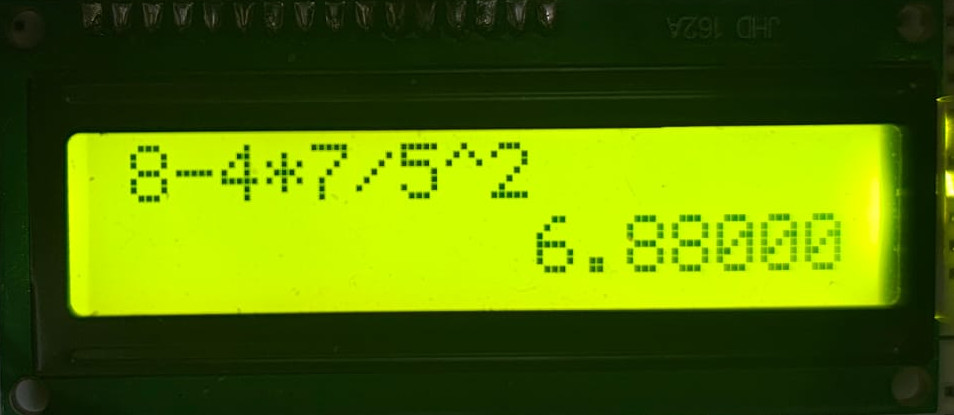
\includegraphics[ width=0.5\textwidth]{./figs/bodmas.png}}
    \hspace{\fill}
    {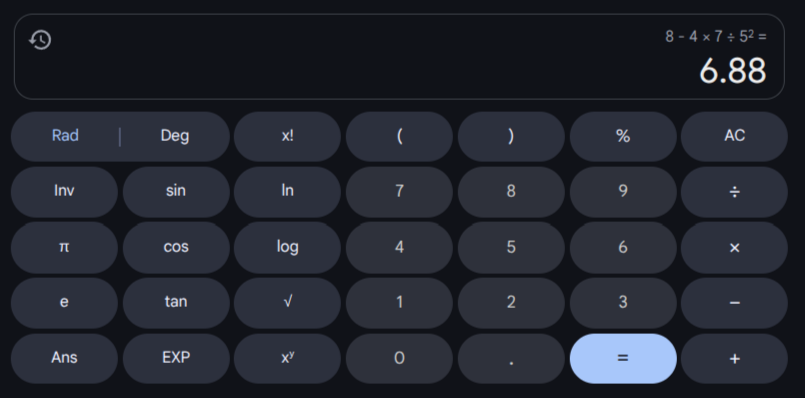
\includegraphics[ width=0.5\textwidth]{./figs/bodmas_calc.png}}
\end{figure*}
\FloatBarrier

\subsection{Trigonometric Functions and Inverse Trigonometric Functions Implementation}
\begin{figure*}[!htb]
    {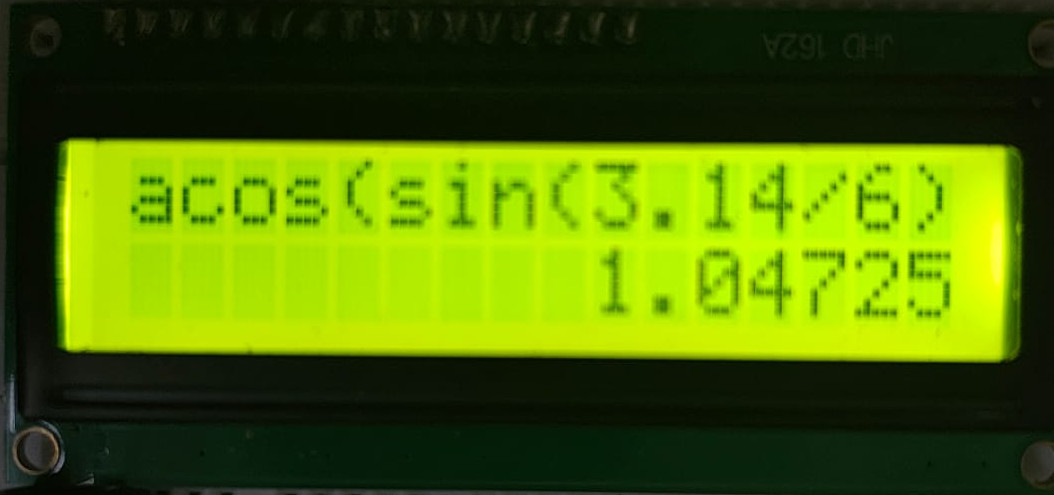
\includegraphics[width=0.5\textwidth]{./figs/trig.png}}
    \hspace{\fill}
    {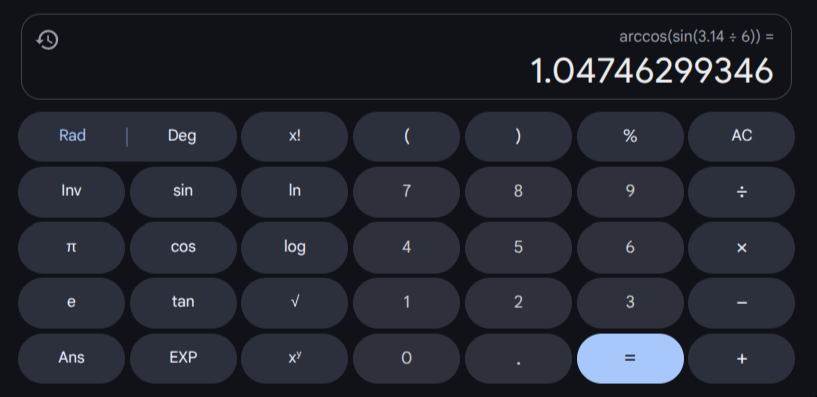
\includegraphics[width=0.5\textwidth]{./figs/trig_calc.png}}
\end{figure*}

\subsection{Power Implementation}
\begin{figure*}[!htb]
    {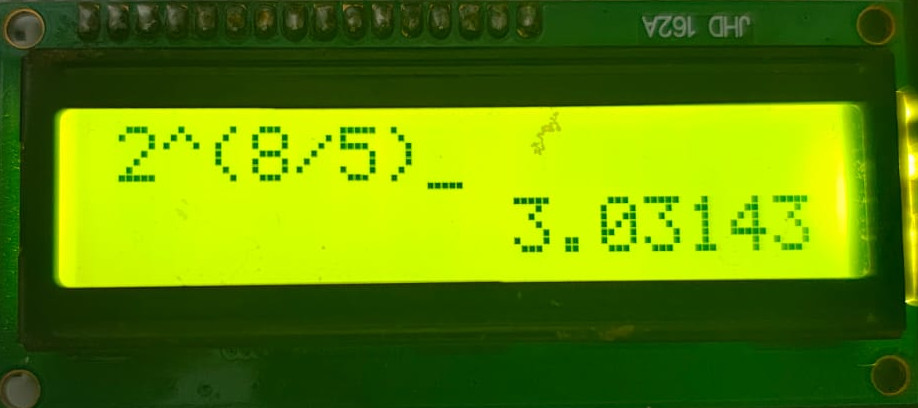
\includegraphics[width=0.5\textwidth]{./figs/pow.png}}
    \hspace{\fill}
    {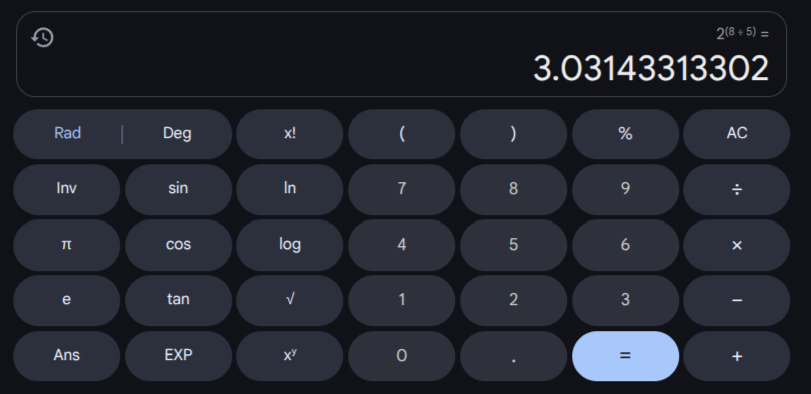
\includegraphics[width=0.5\textwidth]{./figs/pow_calc.png}}
\end{figure*}

\subsection{Natural Logarithm Implementation}
\begin{figure*}[!htb]
    {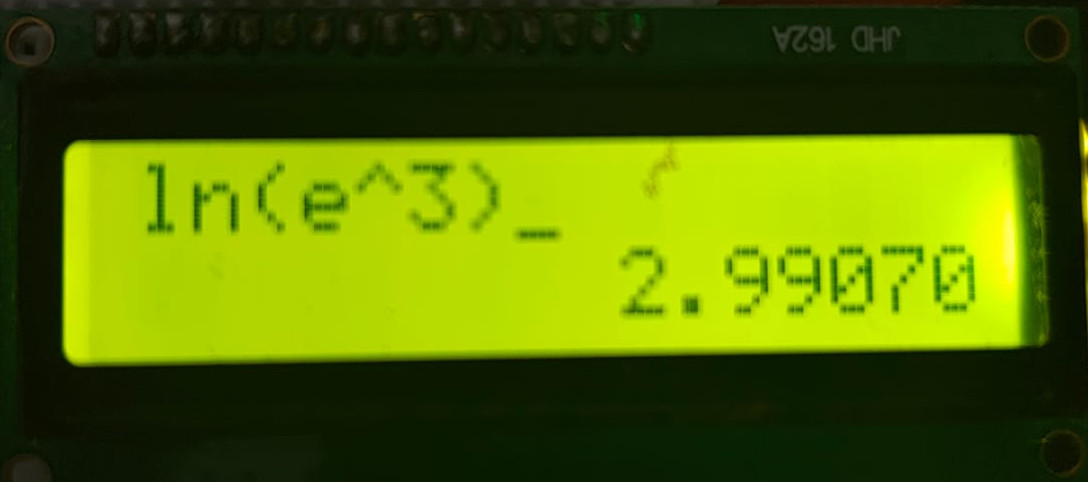
\includegraphics[width=0.5\textwidth]{./figs/ln.png}}
    \hspace{\fill}
    {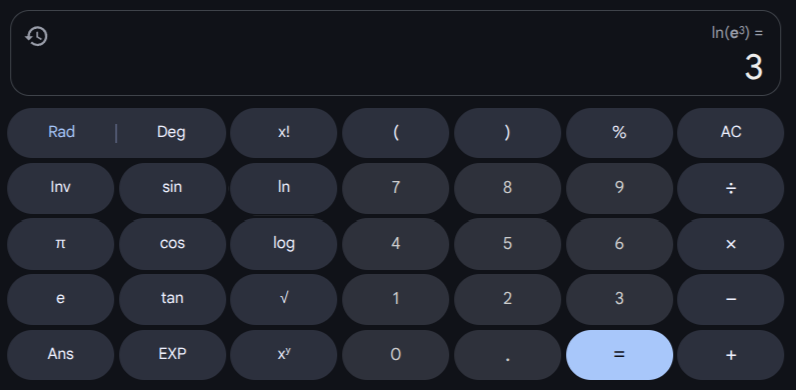
\includegraphics[width=0.5\textwidth]{./figs/ln_calc.png}}
\end{figure*}

\subsection{Logarithm Base 10 Implementation}
\begin{figure*}[!htb]
    {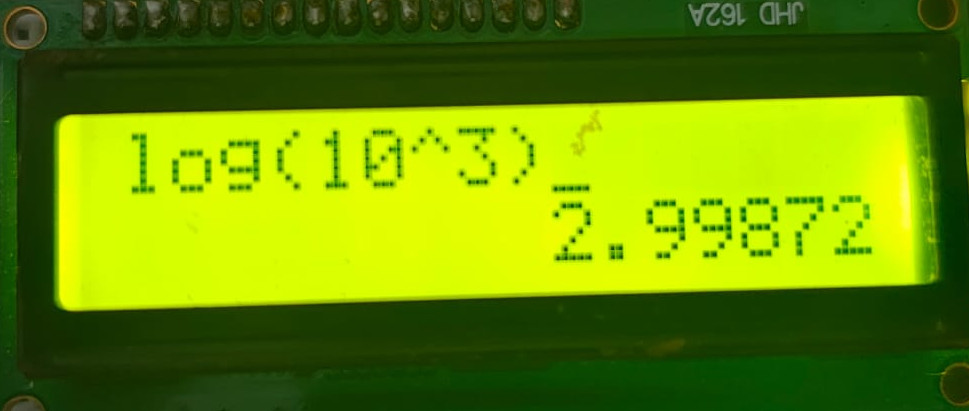
\includegraphics[width=0.5\textwidth]{./figs/log.png}}
    \hspace{\fill}
    {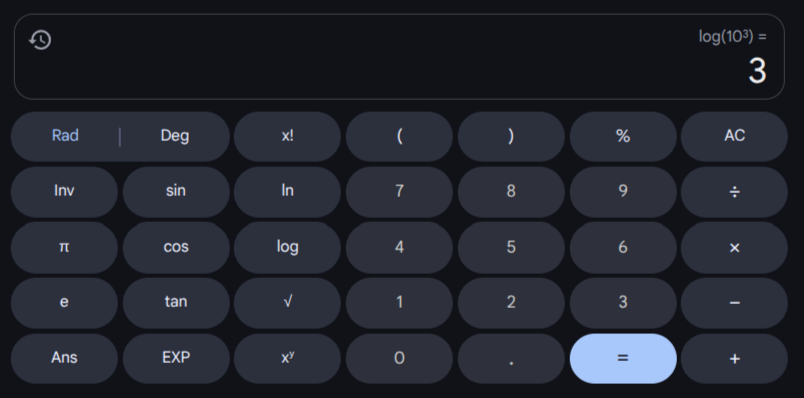
\includegraphics[width=0.5\textwidth]{./figs/log_calc.png}}
\end{figure*}

\section*{Conclusion}
This project shows how I built a working calculator using a button matrix and AtMega328p microcontroller (Arduino Uno) using avr-gcc and differential equations.

\end{document}
